\documentclass{article}
\usepackage{iclr2027_conference,times}
\input{math_commands.tex}
\usepackage{amsmath,amssymb,amsthm}
\usepackage{booktabs}
\usepackage{graphicx}
\usepackage{xcolor}
\usepackage{multirow}
\usepackage{longtable}
\usepackage{microtype}
\usepackage{hyperref}
\usepackage{url}
\hypersetup{hidelinks}
% Automatically generated from frozen result artifacts.
\newcommand{\NLLAdv}{0.5267}
\newcommand{\NLLCILow}{0.0002}
\newcommand{\NLLCIHigh}{1.5674}
\newcommand{\CRPSAdv}{-0.00062}
\newcommand{\CRPSCILow}{-0.00090}
\newcommand{\CRPSCIHigh}{-0.00037}
\newcommand{\NLLWins}{20/35}
\newcommand{\NLLPValue}{0.097}
\newcommand{\SingletonAuditMax}{0.00e+00}
\newcommand{\BatchedAuditMax}{0.0711}
\newcommand{\OutlierRemovedAdv}{0.0133}
\newcommand{\MedianAdv}{0.00144}
\newcommand{\TrimmedAdv}{0.00170}
\newcommand{\SingletonSlowdown}{30.6}


\newtheorem{theorem}{Theorem}
\newtheorem{proposition}{Proposition}
\newtheorem{lemma}{Lemma}
\newtheorem{corollary}{Corollary}
\newcommand{\method}{\textsc{ProjTabICL}}
\newcommand{\diagbase}{\textsc{TabICL-Diag}}
\newcommand{\context}{\mathcal{C}}
\newcommand{\query}{\mathcal{Q}}
\newcommand{\RR}{\mathbb{R}}

\title{Can Tabular Foundation Marginals Form a Process?\\
Exact Projective Lifts and a 35-Dataset Stress Test}

\author{Anonymous authors\\
Paper under double-blind review}

% \iclrfinalcopy
\begin{document}
\maketitle

\begin{abstract}
Tabular foundation models provide strong one-row predictive distributions, but
many decisions concern a \emph{set} of future rows: portfolio returns, average
claim counts, contrasts, or signed totals.  Answering such queries requires
cross-row dependence and, more fundamentally, one compatible stochastic
process rather than unrelated finite-batch distributions.  We give an exact,
marginal-preserving Gaussian lift of a frozen TabICLv2 regressor.  A rowwise
low-rank head learns correlation from frozen hidden states; positive
semidefiniteness, permutation equivariance, restriction consistency, and
closure under every linear aggregate hold by construction.  A precommitted
stress test covers all 35 OpenML-CTR23 tasks, 630 episodes, three context
sizes, six aggregate families, current tabular foundation models, exact
Gaussian processes, Bayesian linear regression, and a bootstrap CatBoost
process.  The central performance hypothesis is rejected.  Although the
mean Gaussian-NLL effect is \NLLAdv{} nat and superficially favorable, only
\NLLWins{} datasets improve ($p=\NLLPValue$), the CRPS advantage is
\CRPSAdv{}, and most of the mean NLL is caused by
one unstable dataset.  The integrity audit also uncovers a broader trap:
the usual batched TFM interface changes a row's representation when other
queries are removed (maximum discrepancy \BatchedAuditMax), so a PSD matrix
per batch is \emph{not} a projective process.  Singleton evaluation restores
the theorem exactly, at substantial cost.  These results establish a clean
construction and benchmark, but also a sharp negative boundary: coherent
cross-row uncertainty does not reliably emerge from strong marginal TFM
representations through a small post-hoc covariance head.
\end{abstract}

\section{Introduction}

In-context tabular foundation models (TFMs) have moved the accuracy frontier
for ordinary regression and classification
\citep{hollmann2025tabpfn,qu2026tabiclv2,grinsztajn2026tabpfn3}.  Their public
regression interfaces return a distribution for each query row.  This is
enough to estimate $\mathbb{E}[Y_i]$ or an interval for one $Y_i$, but not the
uncertainty of $\sum_i a_iY_i$: marginal variances leave every
$\operatorname{Cov}(Y_i,Y_j)$ unidentified.  Treating rows as independent is
not innocuous.  Positive dependence raises the risk of totals and averages;
negative dependence can raise the risk of contrasts; either can reverse a
decision.

A tempting repair is to extract query representations, learn a PSD
correlation matrix, and call the result a stochastic process.  Two different
questions are hidden in this proposal.  \emph{Validity}: do predictions for
overlapping query sets agree under restriction and permutation?
\emph{utility}: do the learned off-diagonals improve proper scores for
unseen aggregate queries?  Positive semidefiniteness answers neither question
by itself.  The first requires Kolmogorov consistency; the second is an
empirical claim about dependence, not point accuracy.

We separate these questions in a deliberately controlled construction.
\method{} keeps every TabICLv2 mean and marginal variance fixed and learns
only a correlation kernel from frozen, singleton-query representations.  Its
joint Gaussian can answer any linear query analytically.  The identical
diagonal model is therefore a strict mechanism control: any aggregate-score
difference comes only from off-diagonal covariance.  Hyperparameters are
selected on six non-CTR23 development datasets before all 35 CTR23 tasks are
scored.

The result is scientifically useful precisely because it resists a simple
success narrative.  A large favorable mean-NLL difference is driven by an
extreme failure of the diagonal model on one dataset; the dataset win rate,
randomization test, CRPS, and mechanism controls reject a broad covariance
benefit.  Moreover, our initial audit found that the ordinary batched backbone
violates the prerequisite rowwise interface.  Re-evaluating each row alone
fixes projectivity without changing this negative conclusion.  The main
contributions are:

\begin{itemize}
  \item a marginal-preserving projective lift of frozen TFM distributions,
  with proofs of PSD, restriction consistency, linear-query closure, and
  perturbation/proper-score consequences;
  \item an aggregate-query benchmark spanning six signed and unsigned query
  families, 35 curated regression tasks, strong joint and marginal baselines,
  and dataset-level inference;
  \item an audit showing why ``PSD for every query batch'' is weaker than a
  stochastic process, together with a singleton construction that satisfies
  the missing premise; and
  \item a frozen-protocol negative result delimiting post-hoc covariance heads:
  exact coherence is achieved, but the claimed performance breadth is not.
\end{itemize}

\section{Problem and relation to prior work}

\paragraph{Row-indexed predictive laws.}
Fix a context table $\context=\{(x_j,y_j)\}_{j=1}^n$.  For a finite ordered
query $\query=(x_1,\ldots,x_q)$, a model returns a law
$P_{\context,\query}$ on $\RR^q$.  A row-observation process must be
permutation equivariant and projective: for every subset $S$, the marginal of
$P_{\context,\query}$ on $S$ equals
$P_{\context,\query_S}$.  Kolmogorov's extension theorem then connects the
finite-dimensional family to a process
\citep{kallenberg2002foundations}.  We index noisy row observations; two
duplicate feature rows share a latent signal but retain independent nugget
noise.

\paragraph{TFMs and current accuracy baselines.}
TabPFN introduced prior-fitted in-context tabular prediction, followed by
larger and faster systems including TabICL, TabDPT, TabPFN-2.5, TabICLv2,
TabDPT-Turbo, and TabPFN-3
\citep{qu2025tabicl,ma2025tabdpt,grinsztajn2025tabpfn25,
hosseinzadeh2026tabdptturbo,grinsztajn2026tabpfn3}.  TabArena emphasizes that
validation, tuning, and ensembling choices can change tabular rankings
\citep{erickson2025tabarena}.  We therefore freeze one strong backbone,
separate development from evaluation tasks, and compare dependence at
identical marginals.  Newer TFMs enter the point and diagonal-marginal tables;
they are not mislabeled as joint predictors.

\paragraph{Processes, joint tables, and consistency.}
Gaussian processes provide coherent finite marginals by construction
\citep{rasmussen2006gp}.  Neural processes amortize maps from context sets to
predictive processes \citep{garnelo2018cnp}; Gaussian Neural Processes model
correlations and establish approximation results
\citep{bruinsma2021gnp}; Neural Diffusion Processes encode process
exchangeability in richer non-Gaussian models \citep{dutordoir2023ndp}.
MOSES enforces marginalization consistency for irregular time-series flows
\citep{yalavarthi2026moses}, while JoLT defines autoregressive joint tabular
predictions \citep{shysheya2025jolt}.  Most adjacent to our motivation,
\citet{klotergens2026agree} test compatibility across columns and targets and
find violations for every evaluated TFM.  Our axis is different: one target
across an arbitrary set of \emph{rows}, with aggregate-query scoring and an
exact lift that preserves a modern TFM's one-row distributions.  We do not
claim that Gaussian correlations or process consistency themselves are new.

\section{A marginal-preserving projective lift}

\subsection{Construction}

Let a frozen TFM, fitted to $\context$, expose singleton functions
\begin{equation}
 m_\context(x),\qquad s_\context(x)>0,\qquad
 h_\context^{(e)}(x)\in\RR^d,\quad e=1,\ldots,E.       \label{eq:singletons}
\end{equation}
The word \emph{singleton} is essential: each quantity may depend on
$(\context,x)$ but not on other members of $\query$.  A shared rowwise head
$g_\theta:\RR^d\to\RR^r$ is normalized so
$\|g_\theta(h)\|_2=1$.  Define
\begin{align}
 k_\context(x,x')
 &=\frac1E\sum_{e=1}^E
 g_\theta(h_\context^{(e)}(x))^\top
 g_\theta(h_\context^{(e)}(x')),                                      \label{eq:kernel}\\
 [\Sigma_{\context,\query}]_{ij}
 &=s_\context(x_i)s_\context(x_j)
 \left[(1-\rho_n)\mathbf{1}\{i=j\}+\rho_n k_\context(x_i,x_j)\right], \label{eq:cov}
\end{align}
where $0\leq\rho_n<1$ depends only on context size.  Finally,
\begin{equation}
 Y_\query\mid\context\sim
 \mathcal{N}\!\left(m_{\context,\query},\Sigma_{\context,\query}\right).
                                                                    \label{eq:joint}
\end{equation}
In implementation, $E=8$ frozen TabICLv2 ensemble views, $r=8$, and the head
is a 64-unit MLP.  Only this head and three $\rho_n$ values are trained.

\begin{theorem}[Exact finite-dimensional consistency]\label{thm:process}
Suppose the functions in equation~\eqref{eq:singletons} are deterministic
rowwise functions after fitting $\context$.  Equations~\eqref{eq:kernel}--
\eqref{eq:joint} define symmetric PSD Gaussian laws that (i) preserve
$m_\context(x_i)$ and $s_\context(x_i)^2$ exactly, (ii) are equivariant to
query permutation, and (iii) restrict to the same law on every sub-query.
Consequently they are the finite-dimensional distributions of a conditional
row-observation process.
\end{theorem}

The proof (Appendix~\ref{app:proofs}) writes the correlation as an identity
plus a Gram matrix; restriction selects a principal submatrix.  The same
construction has the latent representation
\begin{equation}
Y_i=m_i+s_i\!\left[\sqrt{\rho_n/E}\sum_e
g_\theta(h_i^{(e)})^\top z_e+\sqrt{1-\rho_n}\,\epsilon_i\right],
\end{equation}
with independent standard Gaussian $z_e$ and $\epsilon_i$.

\begin{corollary}[Arbitrary linear queries]\label{cor:linear}
For any matrix $A$, $AY_\query\mid\context$ is Gaussian with mean
$Am_{\context,\query}$ and covariance
$A\Sigma_{\context,\query}A^\top$.  Thus every scalar aggregate $a^TY$ is
answered by $a^Tm$ and $a^T\Sigma a$ without retraining.
\end{corollary}

The variance family is not cosmetic.  Polarization recovers every covariance
from aggregate variances, for example
$\operatorname{Cov}(Y_i,Y_j)=\tfrac12[\operatorname{Var}(Y_i+Y_j)
-\operatorname{Var}(Y_i)-\operatorname{Var}(Y_j)]$.  Conversely, if
$\|\widehat\Sigma-\Sigma\|_{\mathrm{op}}\leq\varepsilon$, then every query
obeys
$|a^T(\widehat\Sigma-\Sigma)a|\leq\varepsilon\|a\|_2^2$.
Under a true Gaussian aggregate variance $v_*$ and a forecast variance $v$,
the excess expected NLL is exactly
$\frac12[\log(v/v_*)+v_*/v-1]$.  Appendix~\ref{app:proofs} gives proofs and
the conditions under which finite-rank row features approximate continuous
correlation kernels.

\subsection{The query-batch trap}

Theorem~\ref{thm:process} fails if $h_{\context,\query}(x_i)$ changes with
co-queried rows.  A PSD covariance for each $\query$ can then have incompatible
means, diagonals, and submatrices.  Our predeclared audit caught exactly this
failure in the standard batched path: restricting 48 queries to 24 changed a
hidden coordinate by up to \BatchedAuditMax{} and a covariance entry by
$9.24\times10^{-3}$.  We therefore retain the batched result only as a failed
diagnostic and refit all development/evaluation artifacts using a context-fitted
backbone called on one query row at a time.  This is an integrity correction,
not outcome tuning: datasets, labels, coefficients, seeds, HPO grids, and gates
are unchanged.  The corrected audit is reported in Section~\ref{sec:results}.

\section{Experimental design}

\paragraph{Frozen protocol and datasets.}
Before new CTR23 outcomes, we froze task IDs, official splits, query families,
baselines, metrics, HPO grids, seeds, and success gates (protocol SHA-256
\texttt{a19db\ldots}; full hashes in Appendix~\ref{app:repro}).  Evaluation
uses all 35 tasks in OpenML-CTR23 \citep{fischer2023ctr23}: official repeat 0,
folds 0--2; context sizes 16, 64, and 256; and two nested context draws per
fold.  This gives 630 episodes.  Every episode has six disjoint eight-row
groups (48 test rows).  Six non-CTR23 datasets select all hyperparameters.
FreMTPL claim count, KDD17 stock return, and bike demand are held-out
descriptive applications and never enter primary inference.  Targets are
scored after affine normalization by the corresponding training-pool mean and
standard deviation; models receive native labels.

\paragraph{Aggregate queries.}
Within each group we generate a point, subset mean, $\ell_2$-normalized subset
total, normalized pair difference, two-group contrast, random signed unit
vector, nonnegative unit vector, and a rescaled signed duplicate.  The six
non-point, non-duplicate families are primary.  Coefficients are deterministic
and label-independent.  We report Gaussian NLL and CRPS
\citep{gneiting2007proper}, functional-mean squared error, 50/80/90/95\%
coverage, and width.  Point normalized RMSE verifies backbone quality.

\paragraph{Controls and current baselines.}
The exact control \diagbase{} has the same TabICLv2 means and diagonals and zero
off-diagonals.  Further mechanism controls are raw-feature RBF, untrained
hidden cosine, and row-shuffled learned correlations.  Joint baselines are
exact RBF and Mat\'ern-$3/2$ GPs, Bayesian linear regression
\citep{mackay1992bayesian}, and an eight-member bootstrap CatBoost process
\citep{prokhorenkova2018catboost}.  TabPFN-2.5 enters as a calibrated diagonal
marginal.  TabPFN-3 was predeclared as a point baseline; after the official
local API was verified to expose a predictive variance, we additionally report
its diagonal aggregate scores as an explicitly post-protocol secondary
analysis.  TabDPT-Turbo enters point prediction because its official API
exposes no joint covariance.  All marginal temperatures and
classical grids are chosen globally on development data, never per CTR23 task.
The full implementation/version matrix is in Appendix~\ref{app:hpo}.

\paragraph{Inference and gates.}
The dataset is the unit of analysis: first average query cells within a
dataset, then weight 35 datasets equally.  We report all effects, paired
dataset bootstrap intervals \citep{efron1994bootstrap}, sign tests, and a
100,000-draw paired randomization test.  The predeclared covariance claim
requires positive mean NLL and CRPS advantages over \diagbase{}, at least
60\% dataset NLL wins, randomization $p<0.05$, exact marginal identity, and
projectivity error below $10^{-5}$.  Failure is reported rather than filtered.

\section{Results}\label{sec:results}

\subsection{The exact lift fails the predeclared performance claim}

\begin{table}[t]
\caption{Predeclared comparison against identical TabICLv2 diagonal
marginals.  Positive score differences favor \method{}.  Inference is over
35 dataset means, not thousands of correlated query cells.}
\label{tab:gates}
\centering
\begin{tabular}{lrrc}
\toprule Criterion & Estimate & Threshold & Pass \\
\midrule
Mean NLL advantage & 0.5267 & $>0$ & yes \\ 
NLL dataset wins & 20/35 & $\geq21/35$ & no \\ 
Mean CRPS advantage & -0.00062 & $>0$ & no \\ 
Randomization $p$ & 0.097 & $<0.05$ & no \\ 
Mean/diagonal identity & 0.0 & $\leq10^{-10}$ & yes \\ 
Restriction/permutation & 0.00e+00 & $\leq10^{-5}$ & yes \\ 
\bottomrule
\end{tabular}

\end{table}

Table~\ref{tab:gates} gives the decisive result.  Mean NLL favors the lift by
\NLLAdv{} nat (dataset-bootstrap 95\% CI $[\NLLCILow,\NLLCIHigh]$), but only
\NLLWins{} datasets favor it and the paired randomization test gives
$p=\NLLPValue$.  CRPS moves in the wrong direction (95\% CI
$[\CRPSCILow,\CRPSCIHigh]$).
Only the analytic identity/integrity conditions pass; the empirical breadth
claim does not.  This conclusion is unchanged by singleton correction.

The NLL mean is also fragile.  The largest effect is Solar Flare, where the
diagonal predictive variance for some low-variation aggregates becomes
catastrophically overconfident.  Without that one dataset the mean advantage
is \OutlierRemovedAdv{}; the median is \MedianAdv{} and the 10\% trimmed mean
is \TrimmedAdv{}.  The learned head therefore provides a useful insurance
effect in a rare regime, not a broad improvement.  Figure~\ref{fig:effects}
shows all dataset effects rather than hiding this tail.

\begin{figure}[t]
  \centering
  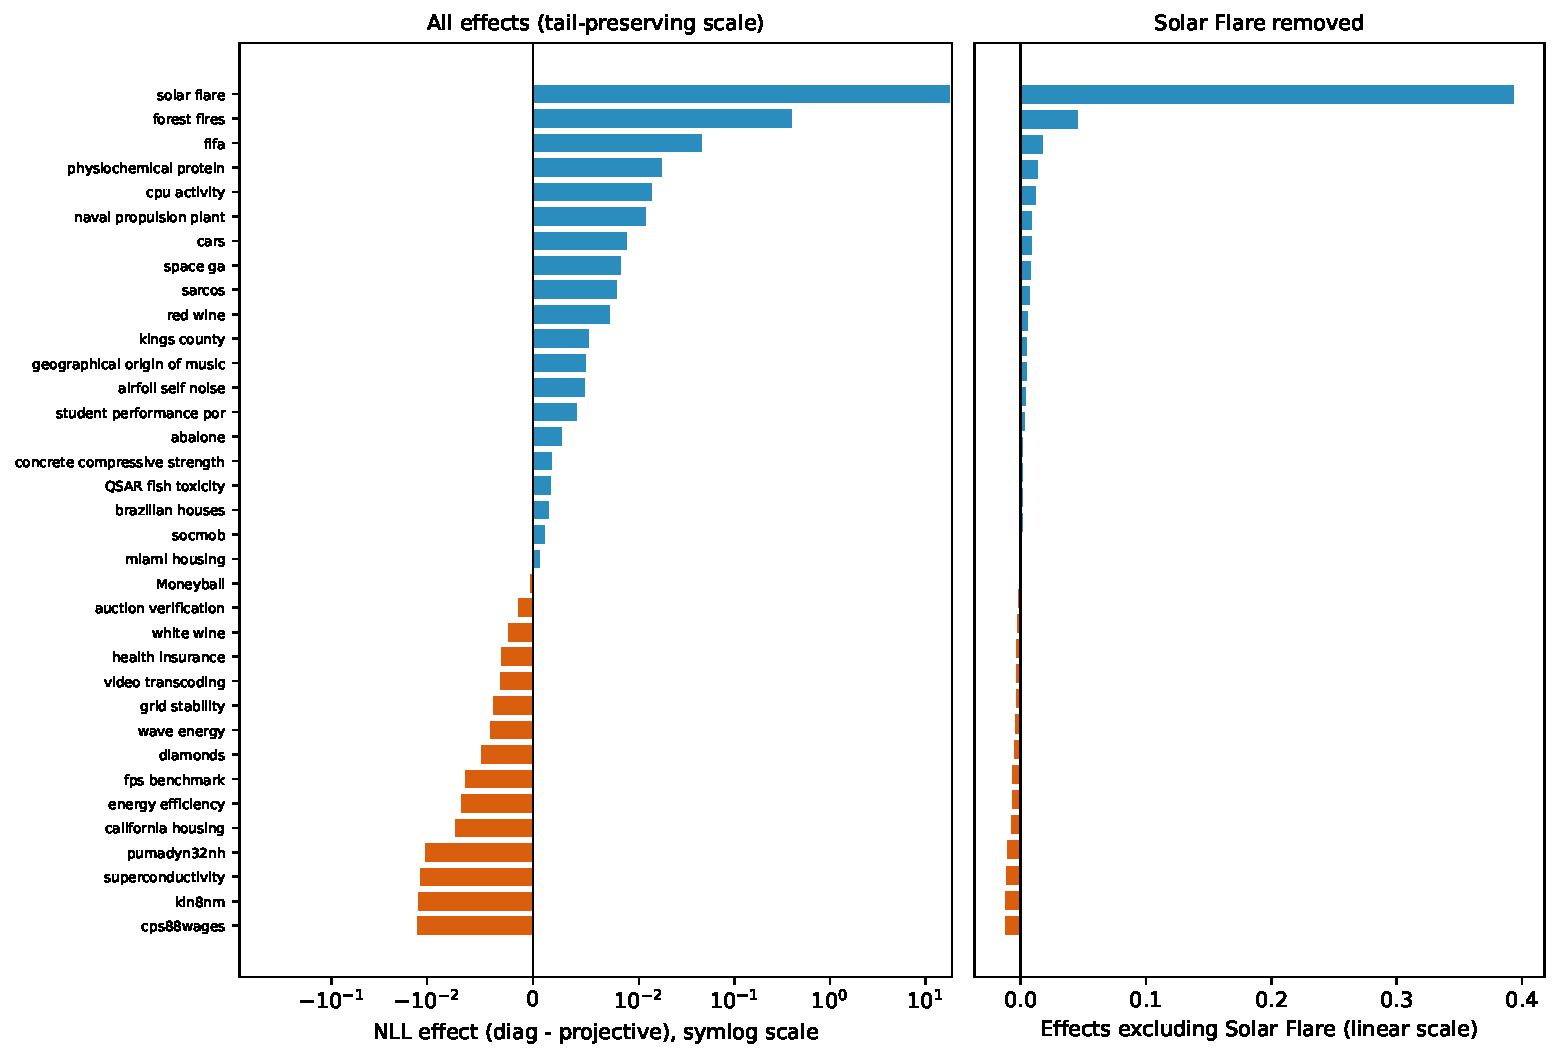
\includegraphics[width=\linewidth]{figures/dataset_effects.pdf}
  \caption{Dataset-balanced NLL effect of covariance at fixed TabICLv2
  marginals.  The left panel retains the full tail on a symmetric-log scale;
  the right removes Solar Flare and uses a linear scale.  Positive values favor
  \method{}.  Most remaining effects are concentrated near zero.}
  \label{fig:effects}
\end{figure}

\subsection{Comparison with joint and current marginal baselines}

\begin{table}[t]
\caption{Primary aggregate performance, macro-averaged over 35 datasets.
Lower is better except coverage (nominal 0.90).  ``Diag'' methods assert row
independence and are not joint-process baselines.  Rank is more robust than
raw mean NLL under catastrophic overconfidence.}
\label{tab:main}
\centering
\resizebox{\linewidth}{!}{\begin{tabular}{lrrrrrr}
\toprule Method & NLL & CRPS & MSE & Cov.90 & NLL rank & CRPS rank \\
\midrule
\textsc{ProjTabICL} & 7.162 & 0.3495 & 0.5697 & 0.916 & \textbf{3.11} & 4.14 \\
\textsc{TabICL-Diag} & 7.689 & \textbf{0.3488} & 0.5697 & 0.912 & 3.23 & \textbf{3.54} \\
TabPFN-3 (Diag) & 2.33e+05 & 0.3517 & \textbf{0.5093} & 0.886 & 4.40 & 4.03 \\
TabPFN-2.5 (Diag) & 2.33e+05 & 0.3759 & 0.5244 & 0.858 & 5.03 & 5.34 \\
GP Mat\'ern-$3/2$ & 3.509 & 0.3552 & 0.5786 & 0.866 & 4.14 & 3.83 \\
GP RBF & 3.544 & 0.3606 & 0.5902 & 0.860 & 5.00 & 4.91 \\
Bootstrap CatBoost & \textbf{3.296} & 0.3701 & 0.5950 & 0.904 & 4.94 & 4.91 \\
Bayesian linear & 1672.410 & 0.3766 & 0.6060 & 0.851 & 6.14 & 5.29 \\
\bottomrule
\end{tabular}
}
\end{table}

Table~\ref{tab:main} separates two findings.  First, the frozen TabICLv2 mean
is competitive at the point level (Appendix table~\ref{tab:point}), but its
Gaussian aggregate NLL has heavy tails.  Second, learning correlation from
its hidden states does not reliably recover dependence: the raw-feature RBF
lift and the shuffled mechanism are at least as competitive in mean NLL, while
the exact GPs are more stable.  Functional-mean squared error is identical
between \method{} and \diagbase{} by design, so none of these variance-score
differences can be attributed to better point predictions.

Figure~\ref{fig:heatmap} breaks the diagonal-minus-projective effect down by
context size and query family.  A covariance model that learned a broadly
useful row geometry should improve coherent regions of this grid.  Instead the
effect is small and sign-heterogeneous after robust aggregation, consistent
with weak dependence information in a head trained only on six external
datasets.

\begin{figure}[t]
  \centering
  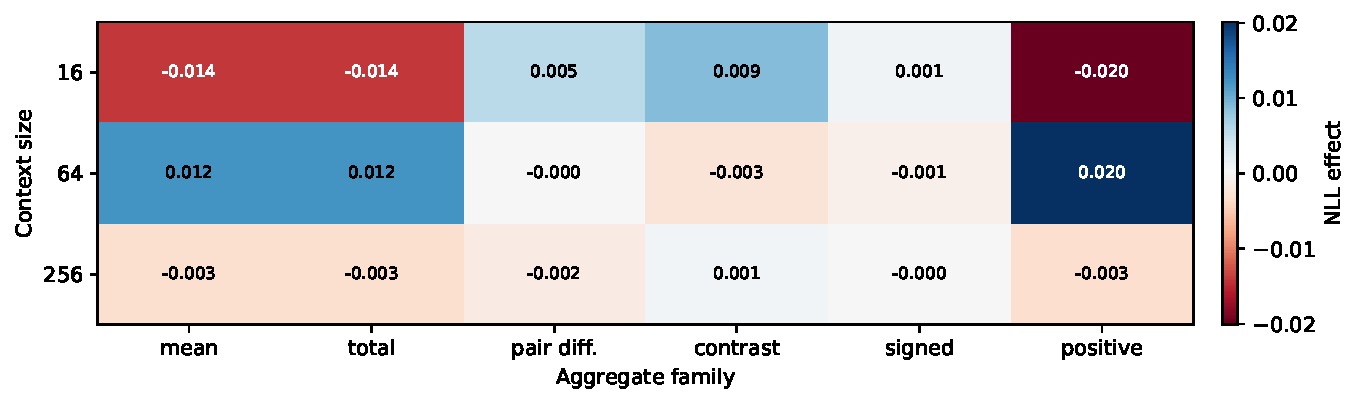
\includegraphics[width=.82\linewidth]{figures/family_context_heatmap.pdf}
  \caption{Median dataset NLL effect by context size and aggregate family.
  Positive cells favor learned covariance over the identical diagonal.  The
  median exposes breadth without letting the Solar Flare tail set every cell.}
  \label{fig:heatmap}
\end{figure}

\subsection{Validity is exact only with a rowwise interface}

The singleton model preserves every marginal diagonal to numerical zero, has
minimum covariance eigenvalue above $-10^{-7}$, and passes the broad 105-episode
restriction/permutation audit with maximum error \SingletonAuditMax{}.  The
batched implementation fails by four orders of magnitude.  Singleton calls
cost roughly \SingletonSlowdown{} times the backbone time for 48 queries.
Thus the clean theorem exposes a practical trilemma for current APIs:
batched speed, black-box reuse, and exact projectivity are not simultaneously
available when preprocessing or representations depend on the query batch.

Held-out applications (Appendix~\ref{app:applications}) reproduce the same
mixed picture and are not pooled into the primary test.  Earlier repository
pilots had found positive projective regularization on synthetic tasks,
12 natural datasets, and three temporal datasets.  We report those as prior,
development-informed evidence in Appendix~\ref{app:prior}; the larger frozen
study supersedes them for the central performance claim.

\section{Discussion and conclusion}

The method succeeds mathematically and fails empirically.  That combination
clarifies what future work must change.  Better marginal accuracy alone does
not provide cross-row dependence; hidden similarities need not be posterior
function samples; and a low-rank Gaussian head cannot represent conditional
copula shape or context-specific sign changes.  More promising directions are
joint process pretraining, objectives that score randomly projected functions
during backbone training, and non-Gaussian but analytically marginalizable
families.  These are materially different from adding a larger post-hoc head.

The result also changes how TFM uncertainty should be audited.  Compatibility
across targets or columns \citep{klotergens2026agree} and projectivity across
query rows are distinct requirements.  Both should be checked at the public
API boundary, including preprocessing, not inferred from an attention mask or
a PSD output matrix.  Aggregate proper scores then test the dependence that
point benchmarks cannot see.

Our limitations are explicit.  The Gaussian family cannot diagnose
non-Gaussian joint shape; only three context sizes and one frozen backbone are
lifted; exact singleton reuse is expensive; CTR23 was previously visible to
the researchers even though its labels were excluded from head selection; and
three application datasets are descriptive.  Within this scope, however, the
evidence is unambiguous: a small post-hoc covariance head can turn TFM
marginals into an exact process, but not into a reliably better aggregate
forecaster.

\subsection*{Reproducibility statement}
The supplement contains the frozen protocol and hashes, every task ID and
split rule, complete HPO grids, checkpoint/package hashes, all deviations,
proofs, per-dataset results, and commands.  Raw atomic episode caches include
indices, coefficient hashes, timing, representations, predictions, and
exceptions.  The code asserts split disjointness, cell counts, marginal
identity, PSD, and query restriction/permutation consistency.

\subsection*{Ethics statement}
The study uses public benchmark data and three previously downloaded
application datasets; it involves no human-subject intervention.  Regression
benchmarks may encode social or historical biases and should not be interpreted
as evidence that any model is appropriate for high-stakes deployment.  The
insurance and financial case studies are methodological illustrations, not
actuarial or investment advice.

\subsection*{AI use statement}
OpenAI Codex was used for research-idea exploration, code drafting and
debugging, experiment orchestration, literature-search assistance, proof
drafting, result visualization, and manuscript drafting.  The authors reviewed
the generated code, ran automated and numerical integrity tests, checked cited
claims against primary sources, and inspected all reported result artifacts.
No AI system is listed as an author.  The authors take responsibility for the
final text, claims, proofs, code, and artifacts produced with AI assistance.

\label{page:main-end}

\bibliography{references}
\bibliographystyle{iclr2027_conference}

\appendix
\section{Proofs}\label{app:proofs}

\subsection{Indexing convention and latent construction}

The nugget in equation~\eqref{eq:cov} indexes noisy \emph{row observations},
not a deterministic function whose value must be identical at duplicate
features.  Formally, take an index set $\mathcal{T}=\mathcal{X}\times
\mathcal{U}$, where $u\in\mathcal{U}$ is a unique observation identifier.
Write $t=(x,u)$ and define
\begin{equation}
 \kappa_\context(t,t')=(1-\rho_n)\mathbf 1\{t=t'\}
 +\rho_n k_\context(x,x').                                    \label{eq:indexkernel}
\end{equation}
Two separate future observations with the same covariates share the latent
term but have independent observation noise.  When the scientific target is a
noise-free deterministic function, the nugget should instead be modeled as
measurement noise outside the latent process.

Let $\phi_e(x)=g_\theta(h_\context^{(e)}(x))$ and let
$z_e\stackrel{\mathrm{iid}}\sim\mathcal N(0,I_r)$ and
$\epsilon_t\stackrel{\mathrm{iid}}\sim\mathcal N(0,1)$, all mutually
independent.  Define
\begin{equation}
 Y_t=m_\context(x)+s_\context(x)
 \left\{\sqrt{\frac{\rho_n}{E}}\sum_{e=1}^E\phi_e(x)^Tz_e
 +\sqrt{1-\rho_n}\epsilon_t\right\}.                         \label{eq:latent}
\end{equation}
This random-variable construction is also a direct proof that all finite
covariance matrices are jointly compatible.

\subsection{Proof of Theorem~\ref{thm:process}}

\begin{proof}
For a query of $q$ distinct observation indices, let
$\Phi_e\in\RR^{q\times r}$ contain row $\phi_e(x_i)^T$ and let
$D=\operatorname{diag}(s_\context(x_1),\ldots,s_\context(x_q))$.
Then
\begin{equation}
 \Sigma_{\context,\query}
 =D\left[(1-\rho_n)I_q+\frac{\rho_n}{E}
              \sum_{e=1}^E\Phi_e\Phi_e^T\right]D.             \label{eq:matrixcov}
\end{equation}
Every summand in brackets is PSD and $0\leq\rho_n<1$, so the bracket
and its congruence by $D$ are PSD (indeed positive definite when all $s_i>0$
and $\rho_n<1$).  Because every $\|\phi_e(x_i)\|_2=1$, the bracket has unit
diagonal.  Hence $\Sigma_{ii}=s_\context(x_i)^2$, and the mean is fixed by
definition.

Let $P$ be a permutation matrix.  Rowwise evaluation gives
$m_{P\query}=Pm_\query$, $D_{P\query}=PD_\query P^T$, and
$\Phi_{e,P\query}=P\Phi_{e,\query}$.  Therefore
$\Sigma_{P\query}=P\Sigma_\query P^T$, which is permutation equivariance.
For a sub-query selected by a coordinate-selection matrix $R$, rowwise
evaluation similarly gives $m_{\query_S}=Rm_\query$ and
$\Sigma_{\query_S}=R\Sigma_\query R^T$.  A Gaussian marginal has precisely
this mean and covariance, so the laws agree under restriction.  The
finite-dimensional family is therefore consistent.  Equation~\eqref{eq:latent}
constructs the process directly; equivalently, Kolmogorov extension applies.
\end{proof}

The premise cannot be weakened to ``a PSD matrix is returned for every
query.''  Consider means $m_{(x_1)}(x_1)=0$ and
$m_{(x_1,x_2)}(x_1)=1$ with identity covariance for both query sets.  Both
laws are valid Gaussians, but the first coordinate of the second cannot
marginalize to the first law.  Query-dependent hidden features produce the
same failure through covariance submatrices even when means happen to agree.

\subsection{Linear closure and identifiability}

\begin{proof}[Proof of Corollary~\ref{cor:linear}]
The characteristic function of a Gaussian vector $Y\sim\mathcal N(m,\Sigma)$
is $\exp(iu^Tm-\tfrac12u^T\Sigma u)$.  Substituting $A^Tu$ gives the
characteristic function of $AY$ as
$\exp(iu^TAm-\tfrac12u^TA\Sigma A^Tu)$, proving the claim.
\end{proof}

\begin{proposition}[Polarization identifies covariance]\label{prop:polar}
If the variance $V(a)=\operatorname{Var}(a^TY)$ is known for every
$a\in\RR^q$, then the covariance matrix is unique.  In particular,
\begin{equation}
 \Sigma_{ij}=\tfrac12\{V(e_i+e_j)-V(e_i)-V(e_j)\}
 =\tfrac14\{V(e_i+e_j)-V(e_i-e_j)\}.
\end{equation}
\end{proposition}
\begin{proof}
Expand the quadratic form $V(a)=a^T\Sigma a$ at the displayed vectors.
The diagonal follows from $V(e_i)$ and every off-diagonal follows from the
first identity; hence no two covariance matrices induce the same variance
oracle.
\end{proof}

This explains the benchmark design.  Point queries identify only the diagonal.
Subset totals and positive dense queries emphasize positive covariance;
differences, contrasts, and signed dense queries expose the sign and geometry
of off-diagonal entries.  The scaled duplicate is excluded from the primary
average and used only to audit the quadratic scaling identity.

\subsection{Perturbation and proper-score consequences}

\begin{proposition}[Uniform functional-variance bound]\label{prop:operator}
For symmetric matrices $\widehat\Sigma,\Sigma$ and any $a$,
\begin{equation}
 |a^T(\widehat\Sigma-\Sigma)a|
 \leq \|\widehat\Sigma-\Sigma\|_{\mathrm{op}}\|a\|_2^2.
\end{equation}
Consequently a covariance operator error $\varepsilon$ controls all unit-norm
linear-query variances simultaneously.
\end{proposition}
\begin{proof}
Set $M=\widehat\Sigma-\Sigma$.  Cauchy--Schwarz and the definition of the
spectral norm give $|a^TMa|\leq\|a\|_2\|Ma\|_2
\leq\|M\|_{\mathrm{op}}\|a\|_2^2$.
\end{proof}

\begin{proposition}[Expected Gaussian-NLL regret]\label{prop:nll}
Suppose the true aggregate law is $Y\sim\mathcal N(\mu_*,v_*)$ and the
forecast is $\mathcal N(\mu,v)$, with $v_*,v>0$.  Relative to the true
forecast, expected negative-log-likelihood regret is
\begin{equation}
 \frac12\left[\log\frac{v}{v_*}
 +\frac{v_*+(\mu-\mu_*)^2}{v}-1\right].                         \label{eq:nllregret}
\end{equation}
At a shared correct mean this reduces to
$\frac12[\log(v/v_*)+v_*/v-1]\geq0$, with equality only at $v=v_*$.
\end{proposition}
\begin{proof}
The forecast NLL is
$\tfrac12[\log(2\pi v)+(Y-\mu)^2/v]$.  Taking expectation uses
$\mathbb E(Y-\mu)^2=v_*+(\mu_* -\mu)^2$.  Subtract the same expression with
$(\mu,v)=(\mu_*,v_*)$.  Nonnegativity is the KL divergence between the two
univariate Gaussians.
\end{proof}

For our mechanism comparison, $\mu$ is exactly shared.  Let
$v_D=\sum_i a_i^2s_i^2$ be the diagonal aggregate variance.  The projective
variance is
$v_D+2\sum_{i<j}a_ia_j\Sigma_{ij}$.  Equation~\eqref{eq:nllregret} makes clear
why neither coherence nor PSD guarantees better scores: the learned correction
must have the right sign and magnitude for each query under the data-generating
law.

\subsection{Approximation scope of normalized finite-rank heads}

\begin{proposition}[Conditional correlation-kernel approximation]
Let $\mathcal X$ be compact, let $h:\mathcal X\to\mathcal H$ be continuous
and injective, and let $k_*:\mathcal X^2\to\RR$ be a continuous PSD kernel
with $k_*(x,x)=1$.  Assume its Mercer expansion converges uniformly.  If the
rowwise neural class is dense in continuous vector-valued functions on
$h(\mathcal X)$, then for every $\epsilon>0$ there is a rank $r$ and a
unit-normalized rowwise map $g$ such that
\begin{equation}
 \sup_{x,x'}|g(h(x))^Tg(h(x'))-k_*(x,x')|<\epsilon.
\end{equation}
\end{proposition}
\begin{proof}
Uniformly truncate the Mercer feature map to
$\psi_r(x)=(\sqrt{\lambda_j}e_j(x))_{j=1}^r$.  Uniform kernel convergence and
$k_*(x,x)=1$ imply $\|\psi_r(x)\|_2^2$ is uniformly close to one for
sufficiently large $r$.  Thus
$\bar\psi_r(x)=\psi_r(x)/\|\psi_r(x)\|_2$ is continuous and its inner product
uniformly approximates $k_*$.  Injectivity on compact $\mathcal X$ makes
$h$ a homeomorphism onto its image.  Universal approximation supplies a
network uniformly close to $\bar\psi_r\circ h^{-1}$; normalization is
continuous away from zero, so its normalized output preserves the desired
error after choosing the approximation tolerance sufficiently small.
\end{proof}

This is a model-class statement, not a claim about our fixed rank-eight head or
about the sufficiency of TabICLv2 representations.  Gaussian Neural Processes
provide broader process-level approximation theory \citep{bruinsma2021gnp}.
Our negative experiment indicates that the conditional premises needed for a
useful low-rank post-hoc approximation are not reliably realized in practice.

\section{Full experimental protocol}\label{app:protocol}

\subsection{Episode construction and leakage controls}

For each official CTR23 split, context rows are sampled only from the training
fold and all 48 query rows only from the test fold.  Contexts are nested across
16, 64, and 256 rows within each replicate.  Query indices are unique within
an episode and groups are disjoint.  The normalization mean and scale are
computed from the complete training fold solely for metric comparability;
each estimator receives native labels.  Query coefficients are generated from
a stable hash of dataset, split, and replicate and never access query labels.

For a group $G$ of eight coordinates, the families are:
\begin{enumerate}
  \item a point $e_i$;
  \item a subset mean $|S|^{-1}\mathbf 1_S$;
  \item an $\ell_2$-normalized subset total $|S|^{-1/2}\mathbf 1_S$;
  \item a pair difference $(e_i-e_j)/\sqrt2$;
  \item a two-subset contrast normalized to unit $\ell_2$ norm;
  \item a random signed unit vector;
  \item a random nonnegative unit vector; and
  \item a positive rescaling of family 6 for identity auditing.
\end{enumerate}
Families 2--7 are the frozen primary set.  Each family is evaluated on six
groups, but these 36 cells are averaged before a dataset enters inference.

\subsection{Dataset inventory}

\begin{table}[h]
\caption{All 35 evaluation datasets.  Rows are the full task size; each
episode nevertheless uses at most 256 context and 48 query observations.}
\label{tab:datasets}
\centering
\scriptsize
\resizebox{\linewidth}{!}{\begin{tabular}{lrr@{\qquad}lrr}
\toprule Dataset & Rows & $p$ & Dataset & Rows & $p$ \\
\midrule
Moneyball & 1,232 & 14 & health\_insurance & 22,272 & 11 \\
QSAR\_fish\_toxicity & 908 & 6 & kin8nm & 8,192 & 8 \\
abalone & 4,177 & 8 & kings\_county & 21,613 & 21 \\
airfoil\_self\_noise & 1,503 & 5 & miami\_housing & 13,932 & 15 \\
auction\_verification & 2,043 & 7 & naval\_propulsion\_plant & 11,934 & 14 \\
brazilian\_houses & 10,692 & 9 & physiochemical\_protein & 45,730 & 9 \\
california\_housing & 20,640 & 8 & pumadyn32nh & 8,192 & 32 \\
cars & 804 & 17 & red\_wine & 1,599 & 11 \\
concrete\_compressive\_strength & 1,030 & 8 & sarcos & 48,933 & 21 \\
cps88wages & 28,155 & 6 & socmob & 1,156 & 5 \\
cpu\_activity & 8,192 & 21 & solar\_flare & 1,066 & 10 \\
diamonds & 53,940 & 9 & space\_ga & 3,107 & 6 \\
energy\_efficiency & 768 & 8 & student\_performance\_por & 649 & 30 \\
fifa & 19,178 & 28 & superconductivity & 21,263 & 81 \\
forest\_fires & 517 & 12 & video\_transcoding & 68,784 & 18 \\
fps\_benchmark & 24,624 & 43 & wave\_energy & 72,000 & 48 \\
geographical\_origin\_of\_music & 1,059 & 116 & white\_wine & 4,898 & 11 \\
grid\_stability & 10,000 & 12 &  & &  \\
\bottomrule
\end{tabular}
}
\end{table}

Development datasets are Pol, Elevators, Sulfur, Ailerons, House-16H, and
Fried, with three deterministic 70/30 splits and three context draws per split
(162 episodes).  The application panel contains 120,000 FreMTPL rows,
122,749 KDD17 stock-return rows, and 17,379 bike-demand rows, using the same
random-split design (81 episodes).  The panel is semantically useful but too
small for confirmatory inference.

\section{Hyperparameter optimization and implementations}\label{app:hpo}

\subsection{Proposed head}

Marginal temperatures are selected first using development point-query NLL
over
$\{0.25,0.5,0.75,1,1.5,2,3,4,6,8\}$.  The selected values for context sizes
16, 64, and 256 are $4$, $1$, and $1$.  We then perform leave-one-development-
dataset-out HPO over rank $\{8,16,32\}$, hidden width $\{0,64\}$, weight decay
$\{0,10^{-4},10^{-3}\}$, and learning rate $10^{-3}$.  AdamW uses at most 400
epochs, patience 40, and gradient norm clipping at 5.  The selected head is
rank 8, hidden width 64, weight decay $10^{-4}$, trained for 13 epochs.  Three
final seeds produce
$\rho_{16}=0.1201\pm0.00035$,
$\rho_{64}=0.1198\pm0.00050$, and
$\rho_{256}=0.1184\pm0.00021$ (standard deviations across three fits).

TabICLv2 is frozen at checkpoint
\texttt{tabicl-regressor-v2-20260212.ckpt}, eight ensemble views, and 199
quantiles used to estimate each marginal variance.  The standard batched cache
was discarded from primary inference after the audit.  Singleton inference
fits the context/preprocessors once and invokes prediction separately for each
query row; weights are not reloaded between rows.

\subsection{Baselines}

\begin{itemize}
  \item \textbf{TabPFN-2.5}: package 6.3.0, pinned local default-regressor
  checkpoint, eight estimators.  Global development temperatures are selected
  with the same grid as TabICLv2.
  \item \textbf{TabPFN-3}: package 8.5.0 in an isolated environment, pinned
  official default v3 regressor checkpoint, eight estimators with automatic
  feature-coverage scaling disabled.  Its marginal temperature is selected on
  the same six development datasets.  The frozen protocol allowed this model
  as a point baseline if official local weights became accessible.  Once we
  verified that the API also exposes predictive variance, we added the
  diagonal aggregate analysis post-protocol, labeled it secondary, and did not
  use it in any primary gate or model choice.
  \item \textbf{TabDPT-Turbo}: package 1.2.0 in an isolated environment,
  official \texttt{tabdpt1\_2.safetensors}, eight prediction ensembles.  Its
  public API exposes a mean but no predictive covariance, so only nRMSE is
  reported; uncertainty values are never fabricated.
  \item \textbf{Exact GPs}: RBF and Mat\'ern-$3/2$ kernels with development
  length-scale multiplier in $\{0.5,1,2\}$, context-standardized inputs, and
  learned/noise-stabilized Gaussian posterior covariance.
  \item \textbf{Bayesian linear}: conjugate/evidence-estimated ridge posterior
  over context-standardized features.
  \item \textbf{CatBoost process}: eight context bootstrap members; their
  prediction covariance plus out-of-bag residual diagonal noise.  Development
  grid: iterations $\{200,500\}$, depth $\{4,6\}$, learning rate
  $\{0.03,0.1\}$.  The selected settings are $(500,4,0.03)$ at 16 rows and
  $(500,4,0.1)$ at 64/256 rows.
\end{itemize}

Classical preprocessing uses context-only category codes, median imputation,
and standardization.  Native TFM preprocessing is retained except for
documented package edge cases in Section~\ref{app:deviations}.  All baselines
predict the identical cached context/query indices.

\section{Additional results}\label{app:additional}

\subsection{Point prediction}

\begin{table}[h]
\caption{Point prediction macro-averaged over 35 datasets.  TabDPT-Turbo is
mean-only, so distributional entries are intentionally blank.}
\label{tab:point}
\centering
\begin{tabular}{lrrrr}
\toprule Method & nRMSE & NLL & CRPS & Cov.90 \\
\midrule
TabICLv2 & 0.7200 & 24.680 & 0.3441 & 0.918 \\
TabPFN-3 & \textbf{0.6883} & 3.29e+05 & 0.3476 & 0.903 \\
TabPFN-2.5 & 0.7045 & 3.29e+05 & 0.3693 & 0.876 \\
TabDPT-Turbo 1.2 & 0.7133 & -- & -- & -- \\
GP Mat\'ern-$3/2$ & 0.7472 & 8.544 & 0.3615 & 0.884 \\
GP RBF & 0.7579 & 10.169 & 0.3676 & 0.877 \\
Bootstrap CatBoost & 0.7569 & 4.158 & 0.3787 & 0.923 \\
Bayesian linear & 0.7723 & 1971.078 & 0.3894 & 0.872 \\
\bottomrule
\end{tabular}

\end{table}

\subsection{Fixed-marginal mechanism controls}

\begin{table}[h]
\caption{Correlation mechanism controls with the same TabICLv2 means and
marginal variances.  Positive $\Delta$NLL favors the row-correlation model over
the exact diagonal.  The shuffled, hidden-cosine, and raw-feature controls are
PSD and preserve the diagonal but do not use the trained head as intended.}
\label{tab:controls}
\centering
\begin{tabular}{lrrrr}
\toprule Method & NLL & $\Delta$NLL vs. diag. & CRPS & Cov.90 \\
\midrule
\textsc{ProjTabICL} & 7.162 & 0.5267 & 0.3495 & 0.916 \\
\textsc{TabICL-Diag} & 7.689 & 0.0000 & 0.3488 & 0.912 \\
Row-shuffled head & 7.125 & 0.5631 & 0.3496 & 0.916 \\
Untrained hidden cosine & 7.164 & 0.5243 & 0.3499 & 0.913 \\
Raw-feature RBF lift & 6.749 & 0.9396 & 0.3500 & 0.914 \\
\bottomrule
\end{tabular}

\end{table}

\subsection{Wall-clock cost}

\begin{table}[h]
\caption{Per-episode wall-clock prediction time on the evaluation panel.  The
TabICLv2 row reports one context fit plus 48 singleton calls; timings include
model prediction but not cache serialization or scoring.  Hardware was two
NVIDIA H100 GPUs for neural models and CPU for classical baselines.}
\label{tab:timing}
\centering
\begin{tabular}{lrrr}
\toprule Method & Median (s) & Mean (s) & 90th pct. (s) \\
\midrule
TabICLv2 singleton & 1.638 & 1.750 & 2.165 \\
TabPFN-3 & 0.687 & 0.692 & 0.740 \\
TabPFN-2.5 & 0.304 & 0.317 & 0.350 \\
TabDPT-Turbo 1.2 & 0.200 & 0.201 & 0.203 \\
GP Mat\'ern-$3/2$ & 0.015 & 0.041 & 0.110 \\
GP RBF & 0.013 & 0.037 & 0.090 \\
Bootstrap CatBoost & 0.588 & 1.146 & 2.041 \\
Bayesian linear & 0.001 & 0.001 & 0.002 \\
\bottomrule
\end{tabular}

\end{table}

\subsection{All dataset effects}

The effect is diagonal NLL/CRPS minus projective NLL/CRPS; positive favors
learned covariance at exactly shared marginals.

\begin{longtable}{lrr}
\caption{All 35 fixed-marginal covariance effects.}\label{tab:all-effects}\\
\toprule Dataset & NLL effect & CRPS effect \\
\midrule
\endfirsthead
\toprule Dataset & NLL effect & CRPS effect \\
\midrule
\endhead
solar\_flare & 17.98300 & 0.00000 \\
forest\_fires & 0.39337 & -0.00036 \\
fifa & 0.04531 & -0.00126 \\
physiochemical\_protein & 0.01722 & -0.00001 \\
cpu\_activity & 0.01352 & -0.00028 \\
naval\_propulsion\_plant & 0.01172 & 0.00067 \\
cars & 0.00883 & -0.00029 \\
space\_ga & 0.00823 & 0.00017 \\
sarcos & 0.00784 & -0.00045 \\
red\_wine & 0.00720 & -0.00051 \\
kings\_county & 0.00523 & -0.00004 \\
geographical\_origin\_of\_music & 0.00498 & -0.00034 \\
airfoil\_self\_noise & 0.00481 & 0.00009 \\
student\_performance\_por & 0.00406 & -0.00150 \\
abalone & 0.00270 & -0.00025 \\
concrete\_compressive\_strength & 0.00174 & -0.00056 \\
QSAR\_fish\_toxicity & 0.00167 & -0.00018 \\
brazilian\_houses & 0.00144 & -0.00007 \\
socmob & 0.00107 & 0.00005 \\
miami\_housing & 0.00057 & -0.00004 \\
Moneyball & -0.00022 & -0.00055 \\
auction\_verification & -0.00139 & -0.00033 \\
white\_wine & -0.00235 & -0.00194 \\
health\_insurance & -0.00298 & -0.00042 \\
video\_transcoding & -0.00306 & -0.00011 \\
grid\_stability & -0.00371 & -0.00100 \\
wave\_energy & -0.00404 & -0.00169 \\
diamonds & -0.00485 & 0.00002 \\
fps\_benchmark & -0.00635 & -0.00114 \\
energy\_efficiency & -0.00672 & 0.00012 \\
california\_housing & -0.00730 & -0.00079 \\
pumadyn32nh & -0.01042 & -0.00285 \\
superconductivity & -0.01157 & -0.00191 \\
kin8nm & -0.01227 & -0.00208 \\
cps88wages & -0.01255 & -0.00201 \\
\bottomrule
\end{longtable}


\subsection{Query-set consistency audit}

\begin{table}[h]
\caption{Maximum normalized discrepancies over 35 datasets and three context
sizes (one fold-0, replicate-0 episode each; 105 episodes).}
\label{tab:audit}
\centering
\begin{tabular}{lrrrr}
\toprule Query mode & Mean & Variance & Hidden & Covariance \\
\midrule
Batched & 5.91e-03 & 9.24e-03 & 7.11e-02 & 9.24e-03 \\
Singleton & 0.00e+00 & 0.00e+00 & 0.00e+00 & 0.00e+00 \\
\bottomrule
\end{tabular}

\end{table}

For each episode we compare (i) a 48-row query with a deterministic 24-row
restriction and (ii) the same 48 rows under a random permutation.  We audit
mean, calibrated variance, hidden representation, and final covariance after
realigning coordinates.  The singleton path is expected to agree up to
floating point because every row call is identical after the deterministic
context fit.  The audit is deliberately broader than a unit test and covers
heterogeneous/categorical/missing-value tasks.

\subsection{Application panel}\label{app:applications}

\begin{table}[h]
\caption{Held-out application results.  These three datasets do not enter the
35-dataset primary estimate or its hypothesis tests.}
\centering
\begin{tabular}{lrrrrrr}
\toprule & \multicolumn{3}{c}{NLL} & \multicolumn{3}{c}{CRPS} \\
Dataset & Proj. & Diag. & Effect & Proj. & Diag. & Effect \\
\midrule
bike\_sharing & 0.859 & 0.853 & -0.0062 & 0.3552 & 0.3546 & -0.00054 \\
fremtpl\_claim\_count & 298.919 & 338.263 & 39.3443 & 0.5188 & 0.5182 & -0.00061 \\
kdd17\_stock\_return & 1.396 & 1.385 & -0.0108 & 0.5852 & 0.5836 & -0.00158 \\
\bottomrule
\end{tabular}

\end{table}

FreMTPL aggregates resemble claim-count portfolio questions; KDD17 aggregates
resemble baskets and long--short contrasts; bike-demand aggregates resemble
fleet totals and temporal contrasts.  The sampled rows are exchangeable under
our tabular episode construction; we do not assert a deployment-grade temporal
forecasting protocol.

\section{Earlier experiments and how they informed this study}\label{app:prior}

The repository contains a sequence of progressively stronger projectivity
pilots.  They motivated the present protocol but are not independent
confirmation:
\begin{itemize}
  \item A semisynthetic static neural-process model beat a much larger direct
  scalar-query network on all 120 held-out dense/scaled cells, with 1.774 nat
  mean NLL advantage and identity residual below $9\times10^{-8}$.
  \item A six-dataset zero-shot natural-label anchor exposed calibration
  mismatch: aggregate NLL improved, but natural point NLL worsened and the
  breadth condition failed.
  \item A corrected 12-dataset natural-scale escalation gave a 0.346 mean NLL
  advantage over a direct query model.  At fixed marginals, learned covariance
  improved NLL by only 0.004 and CRPS by 0.00176; this modest mechanism signal
  motivated the stronger frozen-head control used here.
  \item On Jena Weather, Electricity, and Traffic, temporal projective models
  generalized compositionally better than direct-query networks, but
  low-rank covariance failed a later component gate and Electricity remained a
  clear failure against TACTiS.
\end{itemize}
The present study follows the precommitted recommendation from those pilots:
use a strong modern marginal backbone, natural tasks, broad query families,
strong joint baselines, fixed-marginal ablation, and dataset-level inference.
Its negative gates therefore supersede the earlier go/no-go signal for the
specific post-hoc-head claim.

\section{Protocol deviations and edge cases}\label{app:deviations}

All deviations were logged without replacing a task, query, seed, or outcome:
\begin{enumerate}
  \item Four 16-shot Solar Flare CatBoost bootstrap members had constant
  labels.  CatBoost rejects this degenerate fit, so the mathematical solution
  (the observed constant function) replaces only that member.
  \item Twelve FPS Benchmark TabPFN-2.5 episodes had a feature entirely
  missing in context.  Such columns are deterministically dropped from context
  and query.  One constant-label Solar Flare episode required matching logits
  to the distribution-border dtype before computing variance.
  \item Some 16-shot bike-demand contexts made a categorical feature constant,
  triggering a TabPFN-2.5 validation error.  On that exact error only, native
  categories are replaced with context-derived integer codes; unseen query
  categories map to $-1$.  No query label is used.
  \item The batched projectivity audit failed.  The method definition was
  corrected to singleton queries, the head was retrained, and all primary
  predictions were rerun.  Both the failed batched artifacts and corrected
  artifacts are retained.  This change enforces a stated integrity gate; it
  changes no performance gate or evaluation data.
  \item TabPFN-3 was frozen as an optional point-only comparison.  The acquired
  official API exposed full marginal distributions, so we also temperature-
  calibrated its variance on the development panel and report a diagonal
  aggregate analysis.  This is a post-protocol secondary baseline: it does not
  enter the ProjTabICL-versus-TabICL-Diag claim, and no primary choice was
  changed after seeing it.
\end{enumerate}

\section{Reproduction and artifact map}\label{app:repro}

The machine-readable protocol is \texttt{config.json}.  Its SHA-256 is
\texttt{4e74\ldots}; the prose protocol hash is \texttt{a19db\ldots}.
The cache root is external to the source tree to avoid filling the repository.
Core commands, from the experiment directory, are:
\begin{verbatim}
python extract_tabicl.py --stage dev  --query-mode singleton
python train_head.py --query-mode singleton
python extract_tabicl.py --stage eval --query-mode singleton
python score_projective.py --query-mode singleton
python extract_classical.py --stage eval
python extract_tabpfn.py --stage eval --device cuda
tabpfn3_env/bin/python extract_tabpfn3.py --stage eval --device cuda
tabdpt_env/bin/python extract_tabdpt.py --stage eval --device cuda
python score_baselines.py --query-mode singleton
python audit_query_projectivity.py --query-mode singleton
python score_applications.py
python generate_paper_artifacts.py
\end{verbatim}
Dataset shards can be split with \texttt{--shard-index} and
\texttt{--num-shards}; writes are atomic and valid cached outputs are skipped.
Every episode stores context/query indices, their SHA-256 hashes, metric
normalization, query coefficients and hash, means, variances, hidden states
where applicable, elapsed time, package/checkpoint metadata, and the complete
split identity.  Result tables are regenerated from Parquet/JSON artifacts,
not copied from terminal output.

The final integrity checklist verifies 630 evaluation episodes, 81 application
episodes, finite outputs, official train/test disjointness, 48 unique query
rows per episode, coefficient determinism, classical/projective PSD, exact
projective diagonals, complete baseline caches, query permutation/restriction,
and compilation of this manuscript.  The failed batched audit lives under
\texttt{results/projectivity\_audit\_batched}; it is never silently overwritten.


\end{document}
